\documentclass[12pt]{article}
\usepackage{graphicx}
\usepackage{amsmath}
\usepackage{amsfonts}
\usepackage{subfigure}
\usepackage{fullpage}
\usepackage{footnote}
\usepackage[backend=biber, sorting=none]{biblatex}
\bibliography{oralrefs}
\usepackage{setspace}
\doublespace
%\onehalfspace
\usepackage[font=footnotesize, labelfont=bf]{caption}
\begin{document}
\author{Michael Crumrine}
\title{Searching for Cosmic Inflation with the Bicep Array}
\maketitle



\section{Introduction}

\subsection{A Brief History of Cosmology}
The modern study of cosmology began in 1915 with Einstein's development of the general
theory of Relativity \cite{cite:Einstein}. By combining the Einstein Field
Equations with the assumptions of a homogeneous and isotropic universe,
Friedmann developed a cosmological model in 1922 which forms the core of the standard
model of cosmology \cite{cite:Friedmann}. Hubble's observations in the 1930s
showed an expanding universe \cite{cite:Hubble} providing the first evidence
for a Big Bang origin. This was further supported by the detection of the
Cosmic Microwave Background by Penzias and Wilson in 1965 \cite{cite:Penzias}.



\subsection{The CMB and Inflation}
The Cosmic Microwave Background (CMB) is colloquially called the ``afterglow"
of the Big Bang and is the source of the oldest photons in the universe.
It was originally predicted by Alpher and Gamov in their description of Big Bang
Nucleosynthesis as a consequence of the dense and hot early
universe \cite{cite:BBN}.  In the hot Big Bang, the early universe was an
energetic plasma in which photons scattered continuously from free protons and
electrons which prevented propagation over large distances.  Neutral Hydrogen
was unstable in this period as most photons had energy well above the
ionization threshold for Hydrogen. As the universe expanded, the temperature
of this plasma decreased adiabatically until the free electrons and protons
could combine to form stable, neutral Hydrogen. After this era of
recombination about 380,000 years after the big bang, the photons decoupled
from the plasma and began free streaming through the universe, redshifting due
to continued expansion. We observe these photons today as a 2D ``surface of last
scattering" which follows the spectral distribution of a 2.73K blackbody. 


Increasing experimental precision revealed a uniform CMB and isotropic
universe on scales exceeding the size of the horizon predicted by
Friedmann cosmological models. In 1981 Guth suggested a small period of
exponential expansion to solve these two problems \cite{cite:Guth}. This
theory of \textit{Inflation} has since seen further success in explaining the growth of cosmic structures
as originating from quantum density fluctuations in the primordial projected
to large scales by the inflationary epoch. Inflation also proposes an
explanation for the lack of observed magnetic monopoles and other exotic
relics that many grand unified theories (GUTs) predict would have been
produced at the energy densities in the early universe. Any observable
density of these exotic particles would have been heavily diluted by the
exponential expansion of the inflationary epoch.





\section{Science with the CMB}

\subsection{Mapping the CMB}
Precision cosmology experiments have shown that the CMB is not truly uniform.
Results from COBE in 1992 \cite{cite:COBE} showed the nearly
isotropic temperature spectrum of the CMB contains
fluctuations on the order of 10 $\mu$K. These fluctuations correspond to
density perturbations in the early universe.  We examine the statistical
distribution of these perturbations with the spherical harmonics.


\begin{equation}
	\delta T(\theta,\phi) = \sum _{m=-\ell} ^\ell \sum _{\ell=0} ^\infty
	a_{\ell m}Y_{\ell m}(\theta,\phi)
\end{equation}
The isotropy of the universe prevents the prediction of any individual $a_{\ell
m}$. We therefore take an average over $m$ to form the
angular power spectrum $C_\ell$.

\begin{equation}
	C_{\ell} = \frac{1}{2\ell +1}\sum _{m=-\ell} ^\ell |a_{\ell m}|^2
\end{equation}
Figure \ref{fig:temp_aps} shows the fluctuations in the temperature spectrum
of the CMB as observed by the Planck experiment in their 100 GHz band and the
corresponding angular power spectrum of these fluctuations. The relative sizes
and locations of the peaks in this power spectrum can help constrain
cosmological parameters that describe the composition and evolution of our
universe. 



%The simple $\Lambda$CDM model is based on the six parameters
%shown in Table \ref{table:lcdm6par}. 
\begin{figure}
	\center
	\includegraphics[clip, trim= 1.5in 7.5in 1.5in 1in, width=.4\textwidth, page=9]{planck_map.pdf}
	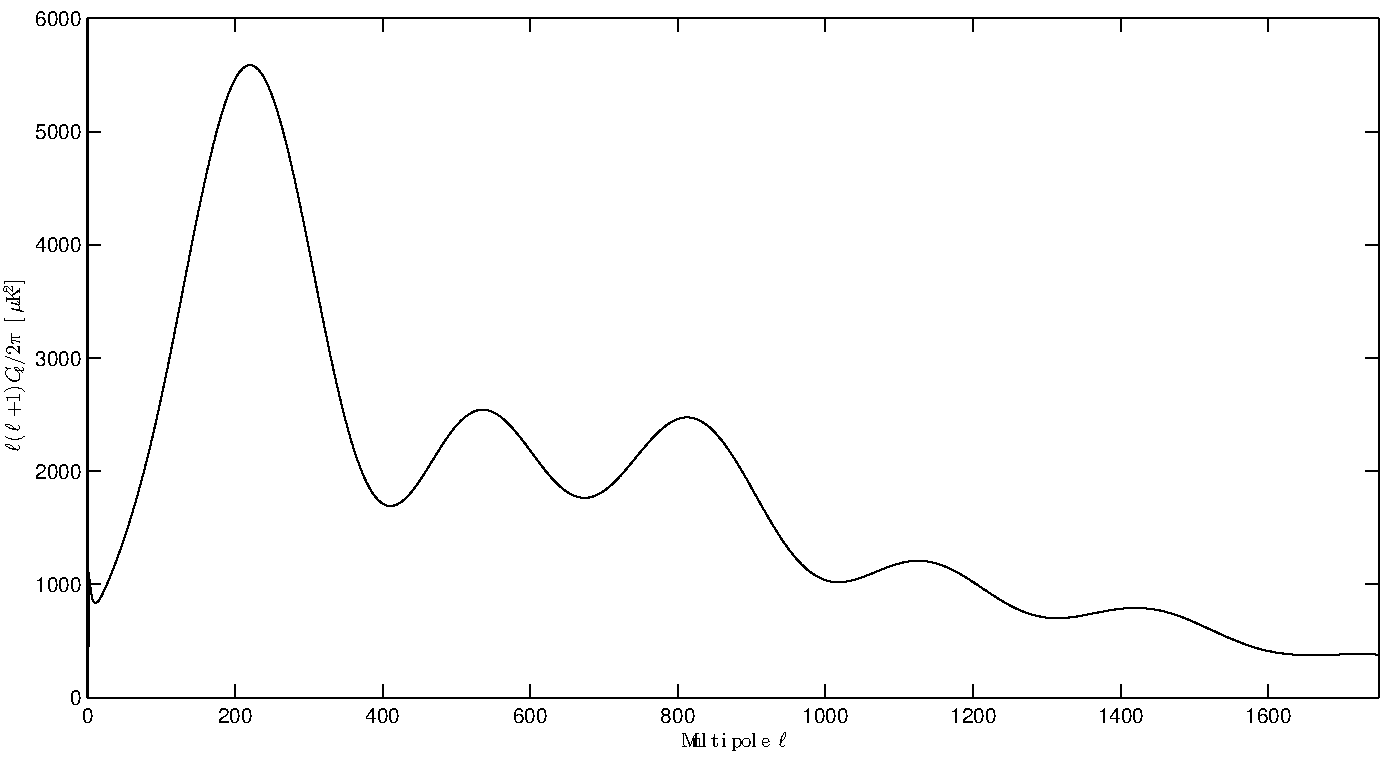
\includegraphics[width=.4\textwidth]{temp_aps.pdf}
	\caption{\textit{Left:} The temperature power spectrum of the CMB.
	\textit{Right:} A map of the temperature fluctuations in the CMB from
	Plank's 2015 results \cite{cite:planckmap}. The primary and acoustic peaks
	in the temperature power spectrum can be used to constrain cosmological
	parameters that describe the geometry, evolution and composition of our
	universe.}
	\label{fig:temp_aps}

\end{figure}



%\subsection{The 6 Parameter Model}

%\begin{table}
%	\center
%\begin{tabular}{|l|l|l|}
%	\hline
%	Parameter & Symbol & Value \\ \hline \hline
%	Baryon Density & $h^2\Omega _b$ &  $0.02240$\\ \hline
%	Cold Dark Matter Density & $h^2\Omega _m$ & $0.1146$ \\ \hline
%	Dark Energy Density ($w=-1$) & $\Omega _\Lambda$ & $0.7181$ \\ \hline
%	Scalar Spectral Index & $n_s$ & $0.9646$ \\ \hline
%	Curvature Fluctuation Amplitude $k_0=0.002$ & $\Delta _\mathcal{R} ^2$ & $2.43
%	\times 10^{-9}$\\ \hline
%	Reionization Optical Depth & $\tau$ & $0.0800$\\ \hline
%\end{tabular}
%	\caption{The six parameters in the simple $\Lambda$CDM
%	cosmological model as shown in the WMAP 9 year results\cite{cite:WMAP9}}
%	\label{table:lcdm6par}
%\end{table}
%
%The first three parameters in Table \ref{table:lcdm6par} - $h^2\Omega_b$, $h^2\Omega _c$, and $\Omega
%_\Lambda$ - describe relative contribution to the composition of our universe
%from baryons, cold dark matter, and dark energy respectively. The matter to
%baryon ratio is related to the size of the first three peaks of the
%Temperature power spectrum in Figure \ref{fig:temp_aps}. The scalar spectral
%index $n_s$ measures the deviation of the power spectrum from the
%scale-invariant case.  The curvature fluctuation amplitude $\Delta
%_\mathcal{R} ^2$ is a
%measure of curvature fluctuation at different angular scales. Finally, the
%reionization optical depth can be used to estimate the damping of CMB
%fluctuations due to the reionization of cosmic baryons which turns the
%universe more opaque for CMB photons.
%WMAP 5yr paper has information on these parameters, so does Dark Universe

%These 6 parameters are largely degenerate with each other in CMB studies
%alone. To break the degeneracies, CMB data is often combined with data from
%other cosmological studies which can set constraints independent of the CMB.
%Studies of Type Ia supernovae use well characterized spectral emissions to create a
%cosmic distance ladder which can constrain the Hubble constant and place
%independent constraints on the composition of the universe. An independent
%measure of these parameters can be made by studying Baryon Acoustic
%Oscillations. The attraction of matter by a primordial overdensity leads to
%increased heat and a large outward pressure. These pressure waves of baryons
%were left behind at fixed radii after photon decoupling leaving a large
%overdensity at the sound horizon. By comparing the overdensities in the CMB
%with the distribution of modern galaxies, BAO places constraints on cosmic
%expansion independent from those set by CMB or supernovae studies.






\subsection{Polarization Anisotropies}
In addition to the temperature anisotropies CMB photons are partially
polarized due to Thompson scattering in a non-uniform temperature field. This
CMB polarization was predicted at the $\approx 10\%$ level by Bond et al
\cite{cite:Bond} and first detected by DASI in 2002 \cite{cite:DASI}. Polnarev
\cite{cite:Polnarev} realized that an inflationary period would imprint an
additional polarization signal on the CMB due to the production of
gravitational waves during the inflationary epoch. The spatial expansion and
compression resulting from a passing gravitational wave would produce a
sufficient temperature quadrupole to impart an additional net polarization on the CMB
photons.



This inflationary gravitational wave (IGW) signal is expected to be orders of
magnitude fainter than the signal due to the temperature fluctuations in the
primordial plasma. Although linearly polarized light is conventionally
described in the Stokes Q, U parameter space, it was shown by Kamionkowski et
al.  \cite{cite:Kamionkowski} that the polarization could instead be
parameterized by a gradient (E-mode) and curl (B-mode) component. The
polarization component due to temperature quadrupoles in the primordial plasma
naturally follows the temperature gradients of the plasma and so produces the
E-mode component. The tensor perturbations due to passing gravitational waves
are not restricted in this way and can therefore create both E-modes and
B-modes. The amplitude of this B-mode signal is characterised by the energy
scale of inflation and related to the E-mode polarization signal by the tensor
to scalar ratio $r$.  Figure \ref{fig:theory_aps} shows the theoretical power
spectra of CMB perturbations in the $\Lambda$CDM standard model of Cosmology
with the addition of an $r=0.1$ IGW B-mode signal. 

As previously mentioned the E, B parameter space is preferred for analyzing
the polarization signal in the CMB as it provides a direct method for
extracting the signal due to inflationary gravitational waves. However, the Bicep /
Keck detectors generate maps in the Stokes Q, U parameter space. By performing
a transformation in Fourier space we can convert Stokes Q and U polarization
into the desired E-mode and B-mode parameter space.





\subsection{Gravitational Lensing}
Although the mean free path of CMB photons is effectively infinite, the
presence of large scale structures in our universe can interact with these
photons and alter the signals we detect in the CMB. In particular,
gravitational lensing due to high matter concentrations is capable of
converting some E-modes into B-modes by relocating polarized photons on the
sky. The transformation from Q and U to E and B occurs in Fourier space and is
inherently nonlocal. The relocation of polarized photons by a gravitational
lens is therefore capable of converting E modes to B modes.
Figure \ref{fig:theory_aps} also shows lensing contribution to the
B-mode angular power spectrum. The lensing contribution to the B-mode spectrum
is largest at small scales due to the high matter densities which produce
strong gravitational lenses. We note also that in principle gravitational
lensing is capable of converting B-modes to E-modes, however the significantly
higher amplitude of the E-mode signal is not highly affected by the addition
of this small signal.



\begin{figure}[ht]
	\center
	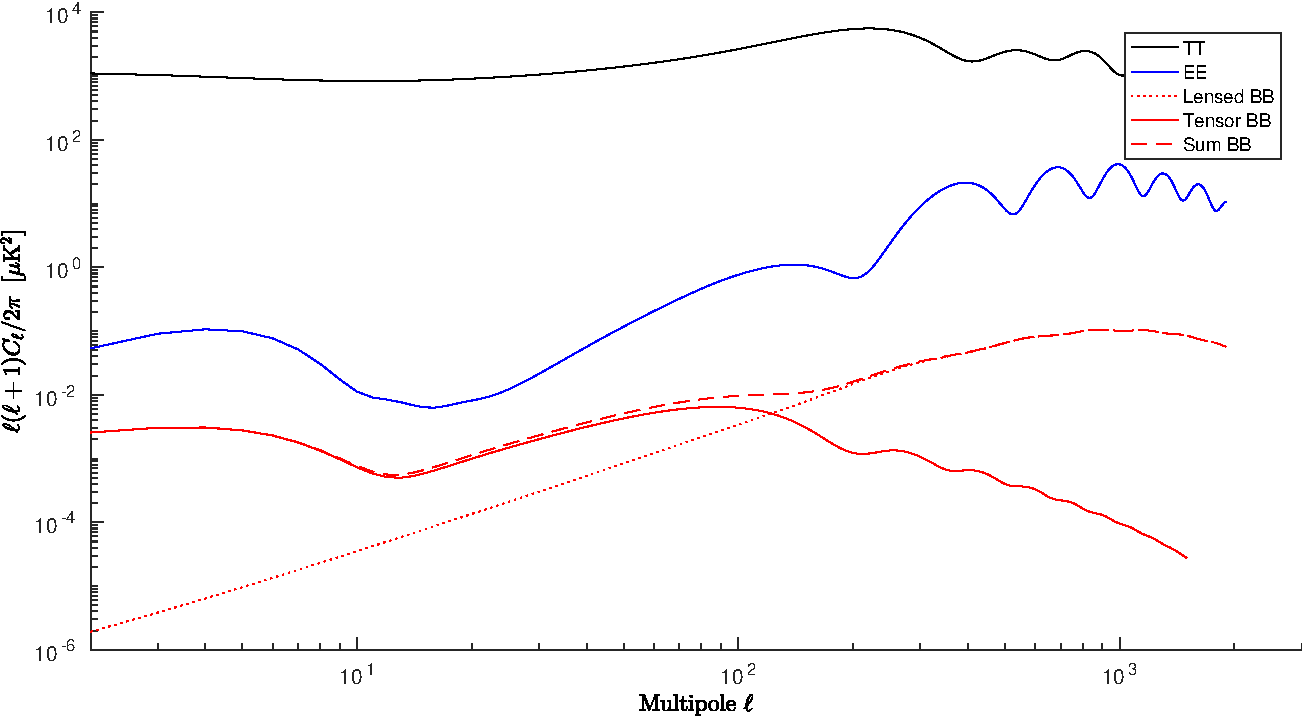
\includegraphics[width=.8\textwidth]{theory_aps.pdf}
	\caption{The CMB power spectrum of the $\Lambda$CDM standard model of
	cosmology as calculated by CAMB using parameters from Planck 2013. The
	temperature anisotropies (black) contain orders of magnitude more power
	than the E-mode (blue) and B-mode (red) polarization anisotropies. The BB
	spectrum is split into a lensing component (dotted) and a tensor component
	(solid) plotted at the $r=0.1$ level. Current constraints on  IGWs
	constrain the signal at less than the $r=0.1$ level shown here. We note
	that some inflationary models predict a tensor to scalar ratio that is
	unobservably small.}
	\label{fig:theory_aps}

\end{figure}


\subsection{Constraints on Inflation}
Although the theory of inflation provides an attractive solution to a number
of problems with the standard big bang cosmology, the exact physics of
inflation are still undetermined. The favored theory of slow roll inflation
proposes a scalar field $\phi$ in which the potential of the field dominates
over its kinetic energy. There mare many possible potentials which fit the
mathematical requirements of inflation theory which yield a range of values
for the tensor to scalar ratio $r$. By continuing to push the constraints on $r$
we restrict the possible potentials of this scalar field. A summary of current
restrictions on inflation in the $r$ and $n_s$ parameter space
shown in Figure \ref{fig:status}. The Bicep / Keck constraints heavily
disfavor the $\phi ^2$ model but still allow for other models which have
$r<0.1$


\begin{figure}
	\resizebox{0.63\textwidth}{!}{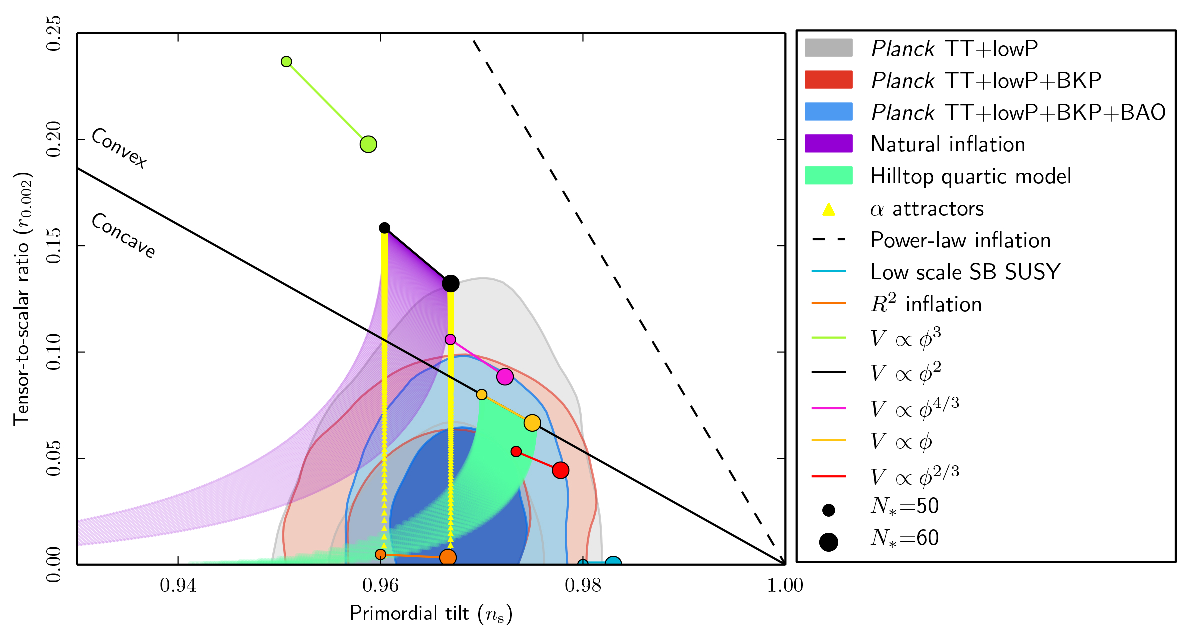
\includegraphics{planck2015XXfig54.pdf}}
	\resizebox{0.36\textwidth}{!}{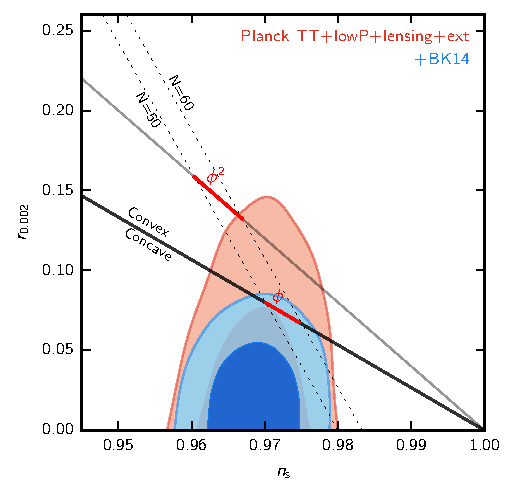
\includegraphics{bk14fig7.pdf}}
	\caption{Left: Reproduced from Planck 2015 XX: "Constraints on
	Inflation"\cite{PlanckXX}
	shows theoretical predictions for select inflationary models in
	the $n_s$,$r$ parameter space and current constraints on those
	parameters. The two dots correspond to different numbers of e-folds.
	Right: Reproduced from BK-VI \cite{BK6} showing improved constraints in this
	parameter space from the latest Bicep / Keck data including a 95GHz band.}
	\label{fig:status}
\end{figure}


\section{The Bicep and Keck Program}
The Bicep and Keck experiments are a staged series of small aperture ground based
telescopes which aim to produce extremely deep degree-scale polarization maps
of the CMB. The high systematics control and long integration time have
enabled Bicep and Keck to set the strictest limits on inflationary
gravitational wave B-mode signals to date. Figure \ref{fig:BK_vs_world} shows
current published measurements of B-mode polarization in the CMB. The Bicep
and Keck experiments along with SPTpol and Polarbear have measured the B-mode
component due to lensing at high significance. Bicep and Keck have currently
published the strictest constraints on B-mode measurements on large angular
scales.

\begin{figure}
	\center
	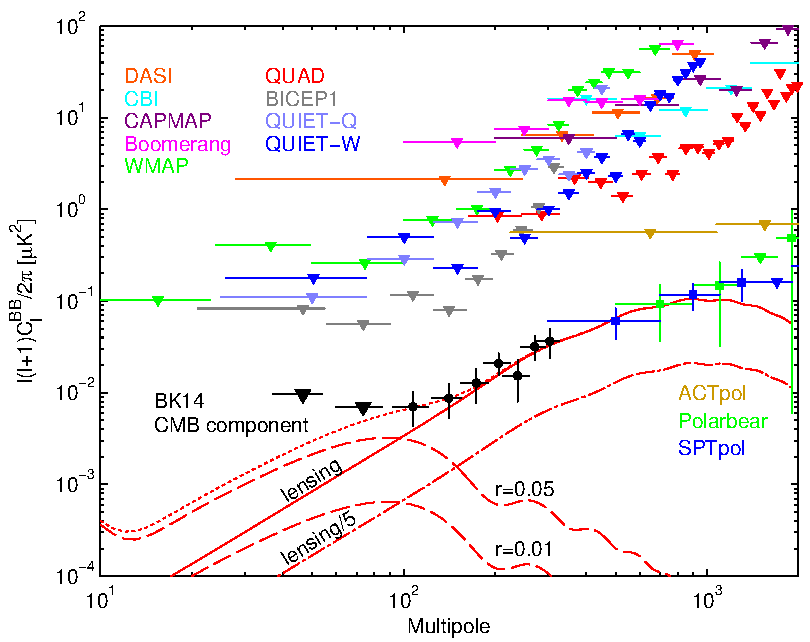
\includegraphics[width=.7\textwidth]{bk14_vs_world.pdf}
	\caption{Published B-mode polarization measurements of the CMB.
	Theoretical predictions for lensing B-modes (solid red) and IGW B-modes
	(dashed red) for two values of r are shown. The SPTpol, Polarbear and
	Bicep/Keck experiments have all recently detected the B-mode lensing
	signal. Bicep and Keck are currently alone in probing large
	angular scales for the IGW B-mode signal}
	\label{fig:BK_vs_world}
\end{figure}


Each generation of receiver builds on the experience gained from
the previous generation while pushing deeper in sensitivity.
Bicep1 was deployed to the south pole in 2006 and used 98 feedhorn coupled
bolometers observing at 100GHz and 150GHz. After observing for three seasons,
Bicep1 established the leading  upper bounds on inflation at $r<0.70$
\cite{cite:Bicep1}. The strategies developed for observation, calibration and
systematics control during the operation of Bicep1 proved the efficacy of
small aperture refractors for CMB polarization studies and have enabled the
high systematics control achieved by subsequent experiments in the series.

Building on the techniques developed with its predecessor, Bicep2 replaced
Bicep1 in 2009. It exchanged feedhorn coupled bolometers for antenna-coupled
transition edge sensor (TES) bolometer arrays developed at JPL which have been
used in every subsequent experiment in the series. Concentrating its observing
power at 150GHz, in March 2014 Bicep2 announced a detection of excess signal
in its observing band consistent with an IGW signal of $r=0.2$\cite{cite:BK1}.
However, the interpretation of this excess as IGW signal relied heavily on
models of polarized dust emission. Later that year new high frequency maps from the Planck experiment
indicated that the dust models had underestimated polarized emission in the
faintest sky regions \cite{cite:PlanckXIX} including the Bicep / Keck
observing patch. A subsequent joint analysis with Planck and cross correlation
between the Planck 353GHz and Bicep2 150GHz maps showed that a substantial
part of the observed excess in Bicep2 was due to polarized dust emissions
\cite{cite:BKP}. Using the new maps of polarized dust provided by Planck, this
joint analysis established a new upper limit of $r<0.12$ \cite{cite:BKP}.

The Keck Array deployed to the south pole in 2012 with five 150GHz receivers
similar to Bicep2. These additional receivers confirmed the excess signal
found with Bicep2 and contributed to the March 2014 results. In addition to
extending the Bicep2 survey depth at 150GHz the Keck Array has extended
observations into three other observing bands at 95GHz, 220GHz and 270GHz.
This extension into other frequencies harnesses the Bicep / Keck program's
proven capability to make deep maps in order to further constrain galactic foregrounds
and refine the models of polarized dust emission. The Keck Array is in its
final observing season with four receivers in the 220GHz band and one at
270GHz.

In the fall of 2014 Bicep3 was deployed at the south pole to run concurrently
with the Keck Array. Bicep3 vastly expands the design of the Bicep2 instrument with a
a larger focal plane with an order of magnitude more detectors and an aperture
twice the size of the Bicep2 receiver. Just as Bicep2 was expanded into the
five receiver Keck array, Bicep3 serves as our pathfinder instrument leading
to the eventual replacement of the Keck Array with the Bicep Array.

The Bicep Array is a funded experiment which will replace the Keck Array for
multifrequency observations. Using the more powerful Bicep3 style receivers,
Bicep array will field four receivers: one each centered at 95GHz and 150GHz,
and two dual band 35/40GHz and 220/270GHz receivers. The new 35/40GHz band will
heavily constrain galactic synchrotron radiation, the upper limits of
which are currently set by WMAP's 23GHZ band and cross correlation with our
own 95GHz band. The addition of the 95GHz and 150GHz receivers will continue
to push sensitivity in the frequencies at which foreground contributions are
expected to be faintest and at the Bicep / Keck maps are already the deepest.
The final high frequency receiver will continue the Keck Array's work in
constraining emissions from polarized galactic dust. Directly observing
these foregrounds in our own observing patch will also eliminate the  need to
account for any spatial variation of the foreground spectra.



\begin{figure}
	\center
	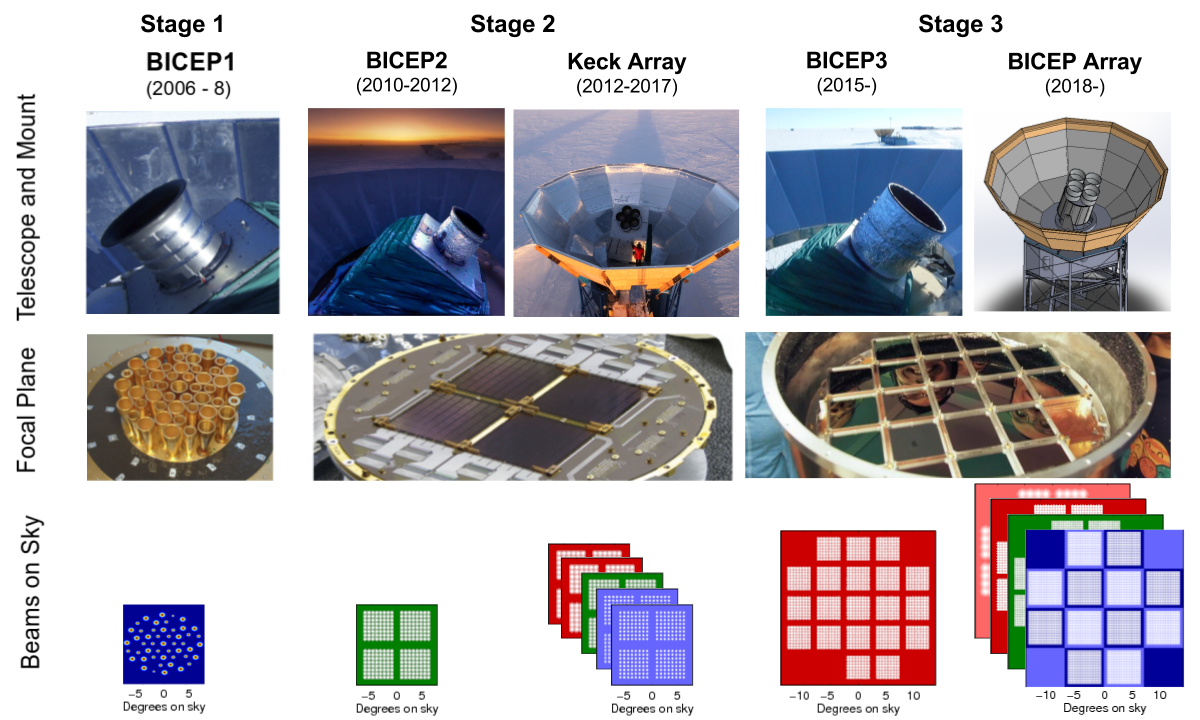
\includegraphics[width=.8\textwidth]{BK_progression.png}
	\caption{The progression of the Bicep/Keck program from Bicep1 to Bicep
	Array. The bottom row shows the beam patterns of the focal planes on the
	sky. With the exception of Bicep1 the focal plane colors correspond to
	band centers of: 35GHz - pink, 95GHz - red, 150GHz - green, 220 GHz -
	light blue, 270GHz - dark blue.}
	\label{fig:BK_progression}
\end{figure}




\section{Multifrequency Observations}

CMB polarization experiments must be able to separate polarized foreground
signals from those imprinted on the CMB. Although these signals can be
minimized by selection of observing area their emissions must be constrained
and accounted for. As shown by the 2014 joint analysis between Bicep2/Keck and
Planck, constraints on these models have significant impact on the
interpretation of any observed excess signal. By expanding observations into
multiple frequencies, the Keck array has begun to constrain these dust
emissions as well as emissions due to galactic synchrotron as shown in Figure
\ref{fig:noilev}.
\begin{figure}
	\center
	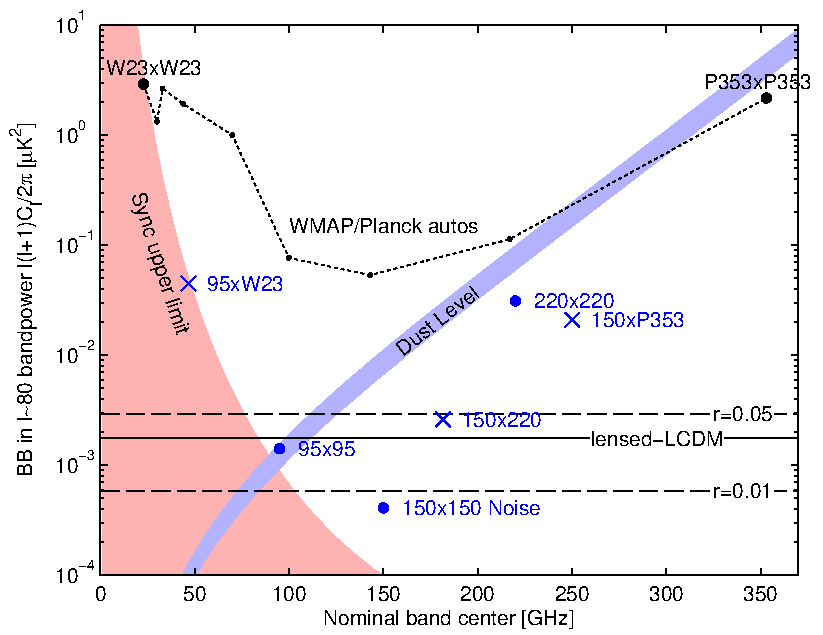
\includegraphics[width=.7\textwidth]{noilev_bk15.pdf}
	\caption{Noise levels in the Bicep/Keck combined observations through the
	2015 observing season. The shaded regions show constraints on the signal
	level of galactic foregrounds and signal levels corresponding to select values
	of $r$ are shown at the bottom. All values are shown in the $\ell=80$
	bandpower where the IGW signal is expected to be maximal (See Figure
	\ref{fig:theory_aps}.)}
	\label{fig:noilev}
\end{figure}

\subsection{Polarized Dust}
Polarized emissions from galactic dust provide an excess B-mode signal on top of
that expected from $\Lambda$CDM and gravitational lensing. These emissions 
are strongly frequency dependent and exhibit a power law like behavior. As shown
in Planck XXII \cite{cite:PlanckXXII} the spectral energy distribution of
galactic dust can be described by a modified blackbody spectrum

\begin{equation}
	I_d=A_d\nu ^{\beta_d} B_{\nu}(T_d)
	\label{eq:dust_sed}
\end{equation}
Where $A_d$ sets the amplitude at a chosen frequency, $\beta _d > 0$ is the spectral
index of dust emission and $B_{\nu}(T)$ is the standard blackbody spectrum. In order
to fully constrain the dust signal we also complement this intensity
spectrum with a description of the dust's power spectral behavior.

\begin{equation}
	D_\ell \propto \ell^\alpha
	\label{eq:dust_aps}
\end{equation}
where $D_\ell=C_\ell \frac{\ell(\ell +1)}{2\pi}$ and $\alpha$ is set
by observation. The parameters in these
equations model the dust contribution to polarization signal in our field. As
Equation \ref{eq:dust_sed} shows this signal is brighter at higher
frequencies. Our current constraints use the Planck 353GHz maps and cross
correlation with our own 220GHz maps to set these dust parameters and
extrapolate to our 95GHz and 150GHz bands. This necessarily means that any
uncertainty contained in the high frequency observations is magnified due to
the exponential frequency dependence.

Figure \ref{fig:noilev} shows the noise uncertainty and signal levels
the $\ell=80$ bandpower where the IGW signal is expected to peak. We are able
to detect signal in excess of that predicted by $\Lambda$CDM with high
significance in our 150GHz band due to the low noise level.
However, the high Planck 353GHz noise as compared to dust signal does not provide
significant enough constraining power to separate dust signal from potential
IGW signal in the 150GHz band. The 220x220 point shows preliminary numbers
from our 2015 observing season in which the Keck array operated with two
220GHz receivers and provides similar constraining power to the Planck 353GHz
data while being closer to our deepest observing bands. Two additional 220GHz
receivers were added for the 2016 observing season and observations at 270GHz
will begin in the current 2017 season. These observations will allow us to
produce continually improving constraints on dust in our field.


\subsection{Galactic Synchrotron}
At low frequencies we must account for polarized galactic synchrotron
emissions. An upper limit for this signal is shown in Figure
\ref{fig:noilev}. Rather than increasing in intensity at higher frequencies,
 galactic synchrotron contributions are strongest at low
frequencies. We model synchrotron emission intensity as
\begin{equation}
	I_\nu = A_s \nu^{\beta _s}
	\label{eq:synch_sed}
\end{equation}
where $\beta _s < 0$ describes the fall off in intensity with frequency and
$A_s$ is the amplitude. The angular power spectrum of galactic synchrotron
follows the same form as dust (Equation \ref{eq:dust_aps}). The points shown
in Figure \ref{fig:noilev} mark the upper limit of synchrotron emissions as
the noise level of current observations in these bands is not sufficient for
detection. Models of the contribution due to synchrotron do not predict
significant contamination at frequencies upwards of 150GHz due to the strong
frequency dependence.

%Look at PIP XXX - might give more information on exactly what this beta
%parameter is. Seems like it might vary with sky patch according to BKP

\section{Bicep Array}

\subsection{Experiment Overview}
Bicep Array will deploy four Bicep3 style receivers in four frequency bands
with first light expected in 2019. Building on the success of previous
experiments, Bicep Array will continue to use the antenna coupled transition
edge sensor (TES) bolometers developed by JPL. These detectors leverage the strong
temperature-dependence of superconductors near their transition temperature to
detect extremely faint signals. Each pixel is composed of two detectors which
are sensitive to orthogonal linear polarizations. By co-locating these
detectors we can use the pair sum to generate intensity maps corresponding to
the CMB temperature and the pair difference to generate the Stokes Q and U
maps.

Each Bicep array receiver will field $\approx$ 10 times the detectors of a Keck
receiver in the same band. With the additional increase in aperture from 26cm to
55cm we will quickly push sensitivity to synchrotron emissions with Bicep Array's new band
and continue to push sensitivity in our deepest 95GHz and 150GHz bands.
Established sensitivities and future projections for the sensitivity of the
Bicep / Keck experiments including the Bicep Array are shown in Figure
\ref{fig:projections}. As we continue to increase in sensitivity to $r$, the
B-mode lensing component will become a significant contributor to the
uncertainty $\sigma _r$.
This achromatic foreground cannot be constrained with multifrequency
observations but it can be accounted for via delensing. Given a high
resolution map of the angular deflection field $\Delta \phi$ of the CMB
photons from last scattering to observation it is possible to undeflect Stokes
Q, U maps of polarized signal and so ``delense" the polarization signal. The
third generation SPT-3G receiver was deployed to the South Pole in late 2016 and
will spend a significant fraction of its time observing the Bicep/Keck sky
patch to aid the delensing effort. In collaboration with SPT-3G we expect to achieve
$\sigma _r <0.005$ by the end of the decade.



\begin{figure}[ht]
	\center
	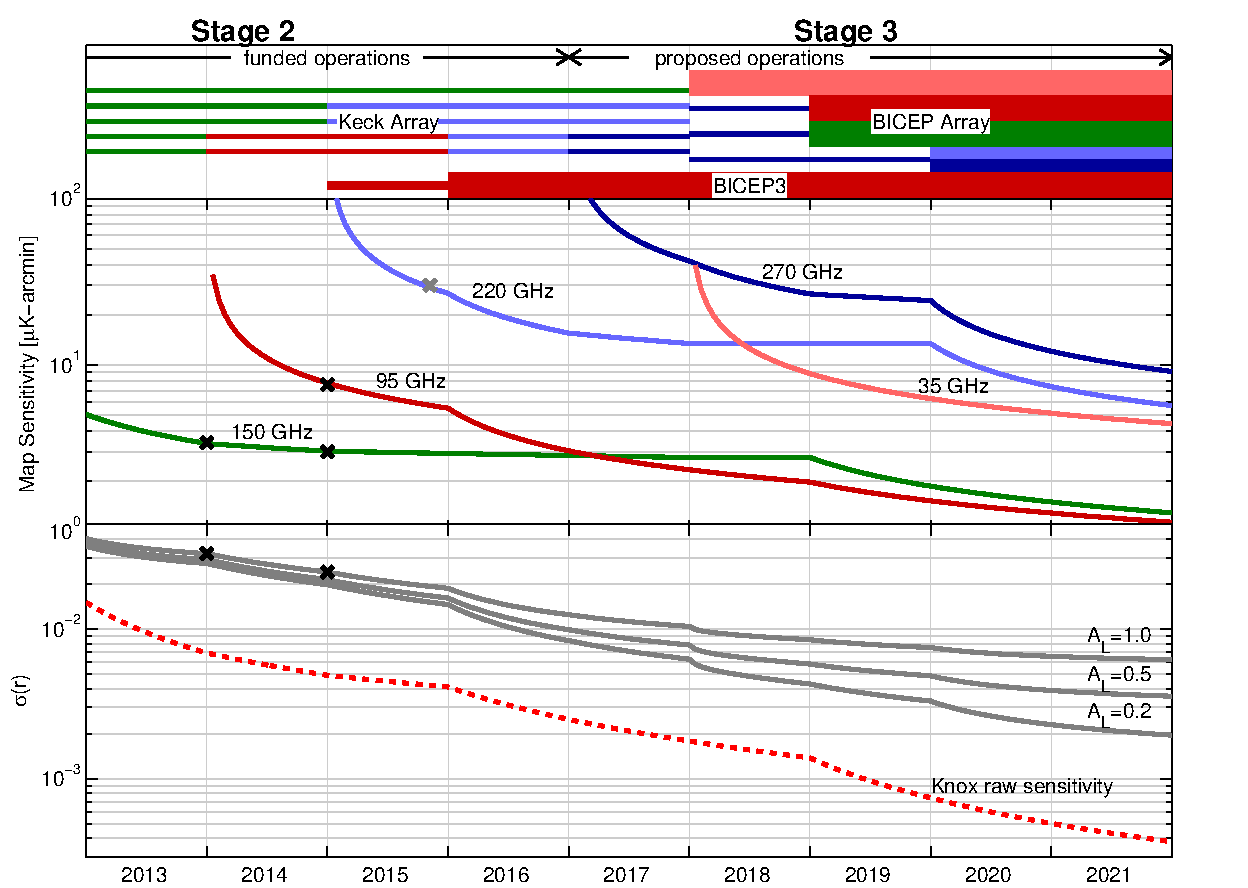
\includegraphics[width=.6\textwidth]{bk_projections.pdf}
	\caption{Projected sensitivity of the ongoing and planned Bicep/Keck
	observational program. The increased throughput of the Bicep array
	receivers will provide increased sensitivity and continue to constrain
	inflation at a rapid rate. \textit{Note: Projections are directly scaled
	from published results and thus include real-world inefficiencies that are
	not reflected in purely theoretical projections. X's mark sensitivities
	achieved in BKP and BK-VI \cite{BK6, cite:BKP}}. Middle: Map depth at each
	frequency as a function of time. Bottom: Sensitivity to $r$ for selected
	levels of delensing efficiency. Performance between $A_L = [0.2, 0.5]$ is
	expected.}
	\label{fig:projections}
\end{figure}


\subsection{Cryogenic Considerations}
The operating temperature of our TES bolometers is around $273$ mK. To reach
these extremely low temperatures, Bicep Array will use a two stage cooling
system composed of a Cryomech Pulse Tube Cryocooler and a second stage Helium
fridge. The cryogenic operating temperatures of our detector and optics
system require a specially designed housing to thermally isolate the focal
plane. As with Keck and Bicep3 the Bicep Array cryostats will consist of 3
nested concentric shells: an ambient temperature vacuum jacket, an
intermediate radiation shield, and a cold optics tube. Hereafter we refer to
these individual stages by their nominal operating temperatures of 300K, 50K
and 4K respectively. This nested approach protects the low temperature optics
from absorbing significant radiative power as $P\propto T^4$.  In addition to
radiation shielding, there is an additional trade-off between structural
support and heat conduction between the temperature shells. A low conductive
loading may introduce significant deviation in pointing direction while a more
structural support system may increase the thermal load on the cooling system. 

\subsection{Thermal Loading}
The cryostat is operated at high vacuum ($\approx 10^{-5}$mTorr) which largely
eliminates conductive loading due to residual gasses. The two largest
contributions are then due to conduction across the structural supports and
radiation from higher temperature stages. Of these, the radiation absorbed by
the lower temperature shells has the highest possible contribution. Radiative
heat transfer for cryogenic systems is a well studied subject. We follow
Ekin's textbook \cite{cite:Ekin} on cryogenic engineering to estimate this thermal load
according to:

\begin{equation}
	\dot{Q}_{h\rightarrow c}=\sigma A_{c} E (T_{h}^4 - T_{c}^4)
	\label{eq:radload}
\end{equation}
where the $h$ and $c$ subscripts denote the hot and cold surfaces
respectively, $\sigma$ is the familiar Stefan Boltzmann constant, and $A_c$ is
the surface area of the cold surface. $E$ is a dimensionless factor that
depends on the emissivity of the surfaces $\epsilon$ as

\begin{equation}
	E=\frac{1}{1/\epsilon _h + 1/\epsilon _c - 1}
\end{equation}
Equation \ref{eq:radload} is valid for parallel plates, and concentric
cylinders assuming the specular reflection regime. Table \ref{table:emis} shows
typical emissivities for the materials used in the Bicep Array cryostats. In
addition to the radiative load, the structural supports conduct heat between
the temperature shells according to the Fourier heat transfer law:


\begin{equation}
	\dot{Q}_{1\rightarrow 2}=\int _{T_1} ^{T_2} \frac{A}{L}K(T)dT
	\label{eq:conduction}
\end{equation}
Where $A$ and $L$ are the cross sectional area and length over which heat is
conducted and $K(T)$ is the thermal conductivity of the material. The large
temperature change across the support struts require a detailed knowledge of
how the materials' thermal conductivity changes with temperature.  NIST
maintains a collection of thermal conductivity measurements for commonly used
materials in cryogenic design including Aluminum and Titanium \cite{cite:NIST}. Bicep Array
uses six Titanium ``V'' shaped supports at the front end to maintain
concentricity of the  optics tube and twelve carbon fiber struts at the back end which support most of the
weight. Carbon fiber as a material is non-standardized which makes determining
the thermal properties difficult, especially at high temperatures where few
conductivity measurements exist. We therefore supplement published low
temperature measurements with direct measurements of conducted power in a test
cryostat system.
\begin{table}
	\center
\begin{tabular}{|l|l|}
	\hline
	\textbf{Material} & \textbf{Emissivity} \\
	\hline \hline
	Rough Aluminum & $\epsilon = 0.07-0.1$ \\
	Polished Aluminum & $\epsilon = 0.04 - 0.06$ \\
	Aluminized Mylar & $\epsilon = 0.035$ \\
	OFHC Copper & $\epsilon = 0.65$ \\ \hline
\end{tabular}
	\caption{Typical emissivity values for materials used in the construction
	of the Bicep Array cryostats.}
	\label{table:emis}
\end{table}



\subsection{Radiation Shielding}
The large surface area of the 50K radiation shield absorbs a significant
amount of power. Using Equation \ref{eq:radload} the raw radiated heat
transfer to the 50K shell from the enclosing 300K vacuum jacket is 86.13W which
is far outside the capacity of our fist stage pulse tube cooling system. To
reduce this load we surround the lower temperature shell with a series of
thermally floating layers of Aluminized Mylar. This multiple layer insulation
(MLI) creates a temperature gradient of isolated radiating shells which
significantly reduces the transmitted power by reducing the $\Delta (T^4)$
term of Equation \ref{eq:radload}. The modified power transmission to the cold
shell when shielded by $N$ layers of MLI is

\begin{equation}
	\dot{Q}_{h\rightarrow c}=\frac{\sigma A_c (T_h^4 - T_c ^4)}{1/\epsilon _h
	+ 1/\epsilon _c -1 + N(2/\epsilon _m -1)}
	\label{eq:mlireduced}
\end{equation}

where $\epsilon _m$ is the emissivity of the MLI. Placing 30 thermally
floating layers in between the 300K vacuum shell and the 50K radiation shield
reduces absorbed radiative power to 0.96W at which point it becomes
subdominant to the thermal loading from the structural supports and the
absorptive optical filters. Although the radiation absorbed by the 4K stage
from the 50K stage is much lower due to the smaller $\Delta (T^4)$ we choose
to include 5 layers of MLI between the 50K radiation shield and the 4K optics
tube as well.


\subsection{Thermal Performance}
Using the equations above we can estimate the thermal loading on each of the
two cryogenic stages of the cryostat and estimate an operating temperature for both
stages of our pulse tube cooling system. We require a 4K stage operating
temperature of less than $\approx 3.5K$ to allow the second stage He fridge to
function. The 50K stage operating temperature is not as crucial, however we
thermally sink optical filters to the 50K radiation shield. Lower
temperatures then allow for cooler optical filters which radiate less power
directly down the optics tube. Using equations \ref{eq:conduction} and
\ref{eq:mlireduced} we calculate the thermal load onto the 4K and 50K stages
as shown below in Table \ref{table:heatload}.

In addition to the thermal load due to radiation from higher temperature
stages and conduction across the structural supports we also account for
conduction across the data cables which read out our detectors and the
radiation absorbed by our optical filters at each stage. The thermal load due
to the optical filters is obtained using data from the Bicep3 experiment's
actual performance. We expect similar performance from Bicep Array which
shares the same aperture size and filtering scheme as Bicep3.



\begin{figure}
	\center
	\begin{tabular}{|l||l||l|}
		\hline
		& \textbf{50K}  & \textbf{4k}\\
		\hline \hline
		Radiation & $2.73 W$ & $0.0479 W$\\
		Bottom Supports & $<2.4 W$ & $0.0759 W$\\
		Top Supports & $1.93 W$ & $0.0821 W$\\
		Data Cables & $1.07 W$ & $0.05 W$\\
		Optical Filters & $12.51 W$ & $0.1538 W$\\
		\hline
		\textit{Total} & $20.64 W$ & $0.4097 W$\\
		\hline
	\end{tabular}
	\caption{Above we show the calculated thermal load on the 50K radiation
	shield and the 4K optics tube due to radiation from higher temperature
	stages, conduction across the structural supports, conduction across the
	data cables and radiation absorbed by the optical filters. The upper limit
	for power conducted across the bottom supports to the 50K radiation shield
	is set by observed performance of the Keck receivers. Note that the
	radiation numbers shown here include power absorbed by all parts of the
	corresponding temperature stages and include absorption from flanges which
	do not have sufficient clearance for an MLI blanket.}
	\label{table:heatload}
\end{figure}


Using these numbers we can estimate the operating temperature of our pulse
tube system by comparing the thermal load with the capacity curve supplied by
the manufacturer shown in Figure \ref{fig:capcurve}. This capacity curve shows
the expected operating temperature of pulse tube's first and second stages -
connected to our 50K radiation shield and 4K optics tube respectively - given
the incident power on both stages. The calculated thermal
load suggests a first stage operating temperature of 39K and a second stage
temperature of 3.2K. While this is sufficient for operation, there is not much
margin. We note however that the Bicep3 pulsetube is oberved to significantly outperform
the Cryomech standard by $\approx 50\%$ on the first stage. This extra
cooling capacity will help to alleviate some of the loading onto the optics
stage by reducing the power transferred to the 4K optics tube.

\begin{figure}
	\center
	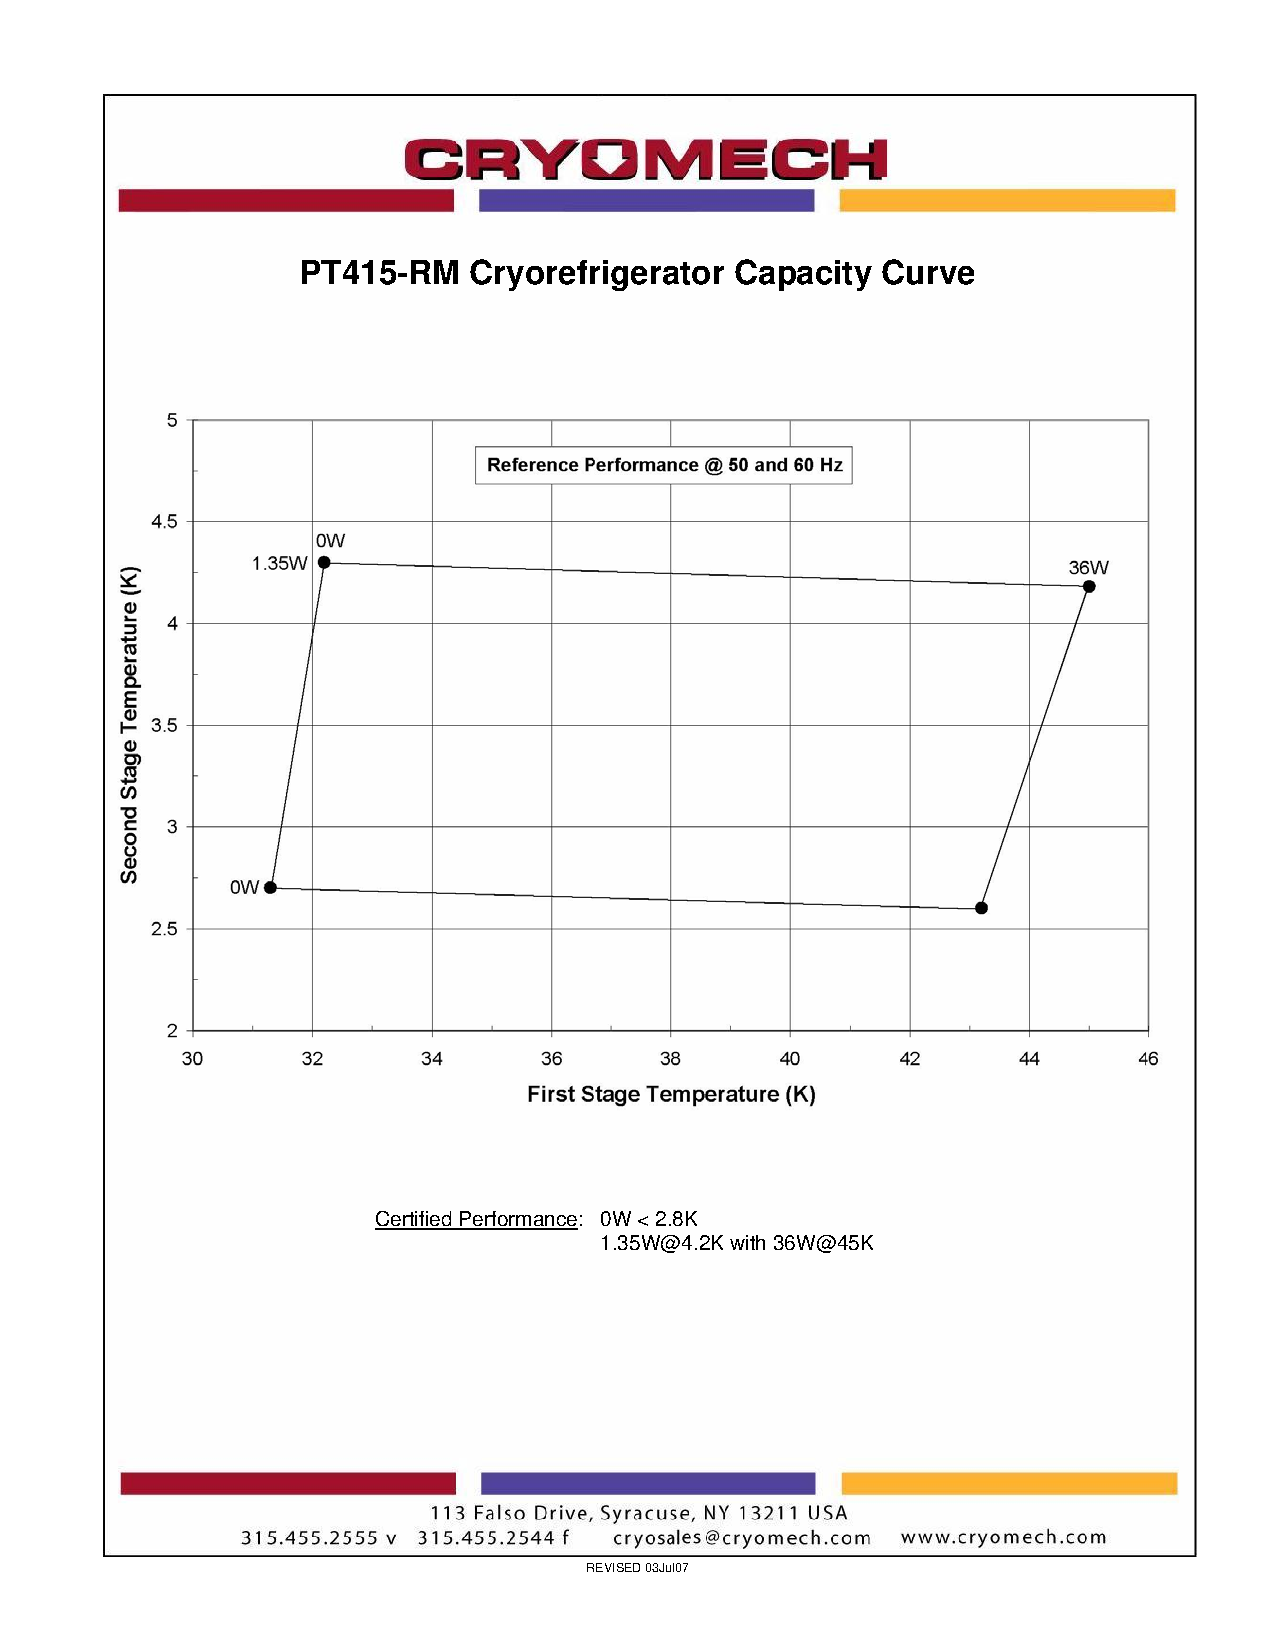
\includegraphics[clip, trim=.8in 3.5in .7in 2.5in,  width=.7\textwidth]{PT415RM_cc.pdf}
	\caption{Reference capacity curve for the PT415 Pulse Tube Cryocooler with
	remote motor option as supplied by Cryomech. The four data points show the
	incident power applied to the first stage (top) and second stage (left).
	Using these points as a reference we can estimate the operating
	temperature of the two pulse tube stages once we have calculated the
	thermal load on each stage. The first stage and second stage of this pulse
	tube cooling system are connected to our 50K radiation shield and 4K
	optics tube respectively. Using the estimated thermal
	load from Table \ref{table:heatload} gives an operating temperature of 39K
	for the first stage and 3.2K for the second stage. The Bicep3 pulse tube
	is observed to significantly outperform the Cryomech standard.}
	\label{fig:capcurve}



\end{figure}



\subsection{Implications for Pointing}
The thermal load is closely tied to the pointing accuracy of the receiver.
Table \ref{table:heatload} shows that heat conduction across the supports is
subdominant only to the thermal load from the optical filters. However, if we
wish to reduce the conductive load across these supports it comes at the cost
of a less rigid support system. To estimate the pointing accuracy of our
optics tube, we use finite element analysis to simulate the deformations of
the cryostat under gravitational load. Figure \ref{fig:pointing} shows the
results of a structural simulation performed with the COMSOL Multiphysics
software suite. In this simulation the cryostat is rotated to our lowest
observing elevation of 45 degrees and the gravitational load of all interior
components are attached to their respective mounting surfaces. 


\begin{figure}
	\center
	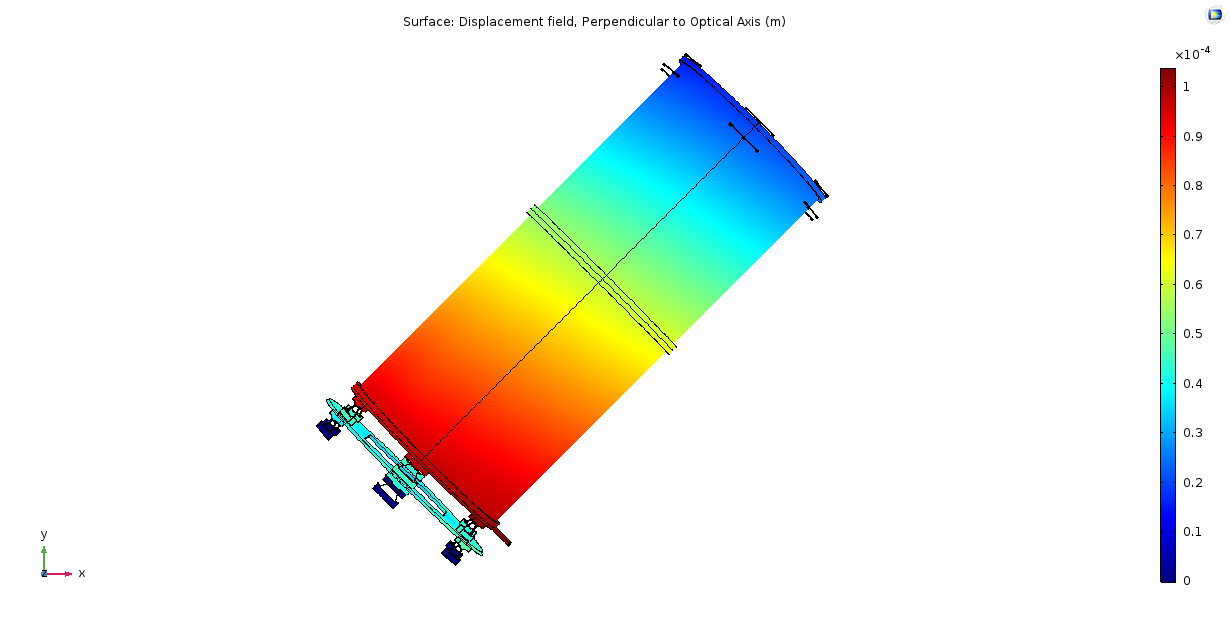
\includegraphics[width=.9\textwidth]{disp_45_perp_4_shell.png}
	\caption{Simulation results of the deformation of the 4K optics tube under
	gravitational load as calculated by the COMSOL simulation suite. The
	colorscale shows the magnitude of deformation in the vector direction
	perpendicular to the optical axis (ie: -45 degrees). The deflections of
	the 50K radiation shield to which the 4K optics tube is attached are
	included in this simulation, however the shield is hidden for clarity.}
	\label{fig:pointing}
\end{figure}



We are most interested in the deformations of the cryostat in the direction
perpendicular to the optical axis. This will give an indication of the shift
in pointing of the optics tube with respect to the fixed outer vacuum jacket.
A simple calculation of the deflection of the back of the optics tube with
respect to the front yields a pointing shift of $10$ arcseconds along the
tube's $1.65$m length. As a secondary check, we also fit a plane to three
points on the deformed plate that supports our focal plane and calculate the angle of the surface normal
to be $45.0028$ degrees from the horizontal corresponding to a $10.255$ arcsecond pointing shift.
The detectors used in Bicep Array will have large beam sizes compared to this
shift with the 270GHz detectors having the smallest beams of 9 arcmin FHWM.
This pointing shift is then acceptable for the Bicep array experiment.



\section{Conclusions}
The Bicep Array experiment will continue the successful achievements of its
predecessors by pursuing increasingly deep maps of the polarized component of
the CMB and expanding these observations into other frequencies in order to
constrain galactic foregrounds. The design of the cryostat is nearing
completion and delivery of the first receiver is expected during the fall of
2017. After careful integration and characterization of the detectors and
readout systems Bicep Array will deploy its first receiver to the South Pole
in the winter of 2018. With a dual band 35/40 GHz focal plane this first
receiver will rapidly push down the upper limits on polarized emission from
galactic synchrotron. Future receivers will continue to push sensitivity in
the bands at which Bicep / Keck have the deepest maps and at which
contribution from galactic foregrounds are dimmest. With delensing in
conjunction with SPT-3G we expect to reach a sensitivity of $\sigma _r <
0.005$ by the end of the decade. This will place significant constraints on
inflationary models and the dynamics of the universe's evolution within the
first instants after the Big Bang.










\printbibliography
\end{document}
